7. По теореме Виета $x_1+x_2=4,\ x_1x_2=\cfrac{q}{2}.$ Тогда $x_1^2+x_2^2=(x_1+x_2)^2-2x_1x_2=16-q=10,\ q=6.$ Параболу $2x^2-8x+6$ построим по трём точкам $(3;0),\ (1;0),\ (2;-2).$
$$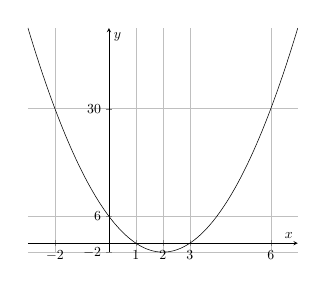
\begin{tikzpicture}[scale=0.5]
\begin{axis}[
    axis lines = middle,
    grid=major,
    legend pos={south west},
    xlabel = {$x$},
    %xlabel style={below right},
    ylabel = {$y$},
    xtick={-2, 1,2, 3, 6},
    ytick={-2,6,30},
               ]
	\addplot[domain=-3:7, samples=100, color=black] {2*x*x-8*x+6};
%\addplot[domain=-3.1:2.5, samples=100, color=red] {70*abs(1-2*abs(abs(x)-2))-10*x^2+10*x-70};
	%\addlegendentry{$\text{Рис. 1}$};
\end{axis}
\end{tikzpicture}$$
